\documentclass[a4paper,15pt, oneside]{book}
\usepackage[italian]{babel}
\usepackage[utf8]{inputenc}
\usepackage[a4paper,top=2.5cm,bottom=2.5cm,left=2cm,right=2cm]{geometry}
\usepackage{amssymb}
\usepackage{amsthm}
\usepackage{graphics}
\usepackage{amsfonts}
\usepackage{amsmath}
\usepackage{amstext}
\usepackage{engrec}
\usepackage{rotating}
\usepackage[safe,extra]{tipa}
\usepackage{multirow}
\usepackage{hyperref}
\usepackage{enumerate}
\usepackage{braket}
\usepackage{marginnote}
\usepackage{pgfplots}
\usepackage{cancel}
\usepackage{polynom}
\usepackage{booktabs}
\usepackage{enumitem}
\usepackage{algorithm}
\usepackage{algpseudocode}
\usepackage{framed}
\usepackage{pdfpages}
\usepackage{pgfplots}
\usepackage{fancyhdr}
\usepackage{caption}
\usepackage{subcaption}
\usepackage{setspace}
\usepackage{hyperref}
\pagestyle{fancy}
\fancyhead[L,RO]{\slshape \rightmark}
\fancyfoot[C]{\thepage}

\title{Modelli probabilistici per le decisioni}
\author{Tommaso Ferrario (\href{https://github.com/TommasoFerrario18}{@TommasoFerrario18}) \\\\
Telemaco Terzi (\href{https://github.com/Tezze2001}{@Tezze2001}) \\\\
Simone Vendramini (\href{https://github.com/simone-vendramini}{@simone-vendramini})}
\date{Marzo 2024}

\pgfplotsset{compat=1.13}

\begin{document}

\maketitle
\newtheorem{teorema}{Teorema}
\newtheorem{dimostrazione}{Dimostrazione}
\newtheorem{definizione}{Definizione}
\newtheorem{esempio}{Esempio}
\newtheorem{osservazione}{Osservazione}
\newtheorem{nota}{Nota}
\newtheorem{corollario}{Corollario}
\tableofcontents
\renewcommand{\chaptermark}[1]{
    \markboth{\chaptername
        \ \thechapter.\ #1}{}}
\renewcommand{\sectionmark}[1]{\markright{\thesection.\ #1}}

\chapter*{Introduction}
\textbf{Deep Learning} is a subset of machine learning that is concerned with 
neural networks that are use to learn underlying features in data.

In general, we can define machine learning as a program that starting from the 
input and the output of a system, learns the rules that govern the system. In 
order to obtain high performance, machine learning algorithms depends heavily on 
the \textbf{representation} of the data. Representation is therefore the fundamental, 
and many artificial intelligence tasks can be solved by designing the right set of features.

The most difference between Deep ML and ML is that, the first one try to learn an
efficient representation of data and than use it to train a learn model. The latter 
one use a representation of data specified by an expert to train a learn model.

Deep Learning use neural networks with many layers of activity vectors as 
representations and learning the connection strengths between that give rise to 
these vectors by following the stochastic gradient of an objective function that
measures how well the network is performing.

So, the key ingredient of deep learning is \textbf{Depth}. There are two main 
ways to measure the depth of a model:
\begin{enumerate}
    \item in terms of depth of the graph describing how concepts are related to
        each other.
    \item in terms of number of sequential instructions that must be executed to 
        evaluate the architecture. This can be influenced by the choice of basic 
        functions used.
\end{enumerate}

One solution to the problem of feature representation is to use machine learning
not only to find the mapping between input and output, but also to find the
representation itself. This approach is called \textbf{Representation Learning}.
The goal of this task is to identify the \textit{factor of variations} that 
explain the observed data. The goal of this task is to identify the factor of 
variations that explain the observed data.

The most common example of representation learning is the use of autoencoders.

A key part of representation learning consists in the \textbf{distributed 
    representation}, which means a many to many relationship between two types
of representation:
\begin{itemize}
    \item Each concept is represented by many neurons.
    \item Each neuron participates in the representation of many concepts.
\end{itemize}

Deep learning solves this central problem in representation learning by introducing
representations that are expressed in therms of other, simpler representations.
An example is bunch of letters form words, sets of words form phrases.

\chapter{Ripasso probabilità}

\begin{definizione}[\textbf{Spazio degli eventi}]
    Lo \textbf{spazio degli eventi} $\Omega$ è l'insieme di tutti gli esisti.
\end{definizione}
\begin{definizione}[\textbf{Evento}]
    Un \textbf{evento} $A$ è un qualunque sottoinsieme di $\Omega$ tale che:
    \begin{equation*}
        A \subseteq \Omega \quad \text{e} \quad P(A) = \sum_{\omega \in A} P(\omega)
    \end{equation*}
\end{definizione}

\begin{definizione}[\textbf{Variabile casuale}]
    Una \textbf{variabile casuale} può essere un'osservazione, un esito o un
    evento il cui valore incerto.
\end{definizione}
L'insieme dei possibili valori che può assumere una variabile casuale è chiamato
\textbf{dominio} o \textbf{spazio degli eventi}.
\begin{definizione}[\textbf{Spazio di probabilità}]
    Uno \textbf{spazio di probabilità} o \textbf{modello di probabilità} è uno
    spazio degli eventi corredato da un assegnamento $P(\omega)$ tale che:
    \begin{equation*}
        0 \leq P(\omega) \leq 1, \quad \sum_{\omega \in \Omega} P(\omega) = 1
    \end{equation*}
\end{definizione}
Si possono creare eventi più complessi combinando gli esiti di diverse variabili
casuali.
\begin{definizione}[\textbf{Evento atomico}]
    Un \textbf{evento atomico} o \textbf{campione} è una specificazione completa
    del valore delle variabili casuali di interesse.
\end{definizione}
Se nel contesto ci sono diverse variabili casuali, il numero di eventi atomici
è la combinazione dei valori tra le singole variabili.

L'insieme di tutti i possibili eventi atomici ha le seguenti proprietà:
\begin{itemize}
    \item \textbf{Mutualmente esaustivo}: non ci sono altri eventi atomici.
    \item \textbf{Mutualmente esclusivo}: può verificarsi solo un evento atomico
          alla volta.
\end{itemize}

\begin{definizione}[Variabile aleatoria]
    Una \textbf{variabile aleatoria} è una variabile che può assumere valori
    diversi in corrispondenza di eventi che costituiscono una partizione dello
    spazio delle probabilità.
\end{definizione}
La teoria della probabilità può essere derivata dalle seguenti assunzioni:
\begin{itemize}
    \item Tutte le probabilità sono comprese tra 0 e 1.
          \begin{equation*}
              0 \leq P(A) \leq 1
          \end{equation*}
    \item Se qualcosa è necessariamente vero allora la probabilità è 1. Un
          ragionamento simile vale per la probabilità nulla.
          \begin{equation*}
              P(\top) = 1, \quad P(\bot) = 0
          \end{equation*}
    \item La probabilità disgiunta che due variabili siano vere si ottiene come:
          \begin{equation}
              P(A \cup B) = P(A) + P(B) - P(A \cap B) \ \equiv \ P(A \lor B) = P(A) + P(B) - P(A \land B)
          \end{equation}
\end{itemize}
\begin{definizione}[\textbf{Probabilità condizionata}]
    La \textbf{probabilità condizionata} rappresenta la verosimiglianza che un
    evento $A$ si verifichi dato che un altro evento $B$ si è verificato.
    La probabilità di $A$ dato $B$ è definita come:
    \begin{equation}
        P(A|B) = \frac{P(A \cap B)}{P(B)}  
    \end{equation}
\end{definizione}
Da questa definizione possiamo dire che le probabilità condizionate riflettono
il fatto che alcuni eventi rendono altri eventi più o meno verosimili. Sempre
in quest'ottica, se un evento non influisce sulla realizzazione di un altro
evento, allora i due sono detti \textbf{indipendenti}. Se due eventi sono
indipendenti allora:
\begin{equation*}
    P(A | B) = P(A)
\end{equation*}
\begin{definizione}[\textbf{Probabilità congiunta}]
    La \textbf{probabilità congiunta}, ovvero il fatto che due eventi si
    verifichino contemporaneamente, si ottiene partendo dalla probabilità
    condizionata e dalle probabilità dei singoli eventi.
    \begin{equation}
        P(A \cap B) = P(A|B) \cdot P(B) = P(B|A) \cdot P(A) \equiv P(A, B) \equiv P(A \land B)
    \end{equation}
\end{definizione}
\begin{definizione}[\textbf{Teorema di Bayes}]
    Il \textbf{teorema di Bayes} è un'importante relazione tra probabilità
    condizionata e probabilità congiunta. Esso afferma che la probabilità di
    un evento condizionato ad un altro evento può essere calcolata in termini
    della probabilità dell'evento condizionante e della probabilità
    condizionata dell'evento di interesse.
    \begin{equation}
        P(A|B) = \frac{P(B|A) \cdot P(A)}{P(B)}
    \end{equation}
    \begin{proof}
        La dimostrazione del teorema di Bayes si ottiene partendo dalla
        definizione di probabilità condizionata e dalla probabilità congiunta.
        \begin{equation*}
            P(A \cap B) = P(A|B) \cdot P(B) = P(B|A) \cdot P(A)
        \end{equation*}
        Da cui si ottiene:
        \begin{equation*}
            P(A|B) = \frac{P(B|A) \cdot P(A)}{P(B)}
        \end{equation*}
    \end{proof}
\end{definizione}
Un altro modo di interpretare la regola di Bayes è quello di considerare
gli eventi come cause non necessariamente osservabili. In questo caso, la
verosimiglianza degli effetti osservabili date le cause non osservabili, in
formule:
\begin{equation*}
    P(\text{causa}|\text{effetto}) = \frac{P(\text{effetto}|\text{causa}) \cdot
        P(\text{causa})}{P(\text{effetto})}
\end{equation*}
La regola di Bayes ci permette di usare questo modello per inferire la
verosimiglianza della causa nascosta data l'osservazione dell'effetto.

Una semplificazione, che può tornare utile in determinate condizioni, della
regola di Bayes si può fare se si conosce la $P(E|C)$ per ogni causa $C$. In
queste condizioni possiamo evitare di conoscere $P(E)$.
\begin{equation}
    P(C|E) = \frac{P(E|C) \cdot P(C)}{\sum_{i} P(E|C_i) \cdot P(C_i)}
\end{equation}
Questa procedura consiste nel normalizzare le probabilità condizionate.
\begin{nota}
    È importante osservare che la regola di Bayes confida nel fatto che l'effetto
    deve essere scaturito a causa di una delle cause ipotizzate. Se ci sono altre
    cause non considerate, la regola di Bayes non è applicabile.
\end{nota}
Il significato del teorema di Bayes può essere espresso come: apprendere
attraverso l'esperienza.

Posso riassumere nella seguente formula:
\begin{equation}
    P(A|B) = \alpha \cdot P(B | A) \cdot P(A)
\end{equation}
dove:
\begin{itemize}
    \item $P(A)$ è la probabilità a priori di $A$.
    \item $P(B|A)$ è la verosimiglianza di $B$ dato $A$.
    \item $P(A|B)$ è la probabilità a posteriori di $A$.
    \item $\alpha$ è un fattore di normalizzazione.
\end{itemize}

Supponiamo ora di voler combinare diverse variabili casuali. Siccome abbiamo
più effetti il nostro modello causale diventa complicato. Ad esempio se abbiamo
$N$ effetti booleani ci saranno, data una causa, $2^N$ diverse combinazioni
di evidenze che dobbiamo modellare.

Questo porta a un notevole aumento della complessità del modello. Per ridurre
questa complessità, la probabilità congiunta di un insieme di eventi può essere
espressa come una \textbf{catena di probabilità condizionate}.
\begin{definizione}[\textbf{Catena di probabilità condizionate}]
    Una \textbf{catena di probabilità condizionate} è una sequenza di probabilità
    condizionate che rappresenta la probabilità congiunta di un insieme di eventi.
    \begin{equation}
        P(A_1 \cap A_2 \cap \ldots \cap A_n) = P(A_1) \cdot P(A_2|A_1) \cdot
        P(A_3|A_1 \cap A_2) \cdot \ldots \cdot P(A_n|A_1 \cap \ldots \cap A_{n-1})
    \end{equation}
\end{definizione}
Questo approccio risulta utile per fare \textbf{inferenza}. Consideriamo un
insieme di eventi $E_1, E_2, \dots, E_n$ e tutte le possibili combinazioni dei
loro valori, per semplicità usiamo $\top, \bot$. Inoltre, conosciamo tutti i
valori $P(E_1, E_2, \dots, E_n)$ e supponiamo che un sottoinsieme di questi
presenti un valore definito, come ad esempio $E_j = Vero = e$.
Chiamiamo \textbf{inferenza probabilistica} il processo di calcolo del valore:
\begin{equation}
    P(E_i = Vero|E_j=e)
\end{equation}
In generale l'inferenza probabilistica non è trattabile usando questo metodo 
perché avendo $N$ eventi binari, dovremmo avere una lista di $2^N$ probabilità congiunte.
Si riduce il numero utilizzando metodi approssimativi, qualitativi o sfruttando 
l'indipendenza condizionata. 
\chapter{Reti Bayesiane} \label{cap:RetiBayesiane}
\section{Introduzione}
Le reti bayesiane sono un \textbf{modello grafico probabilistico} che rappresenta
le relazioni probabilistiche tra un insieme di variabili. Queste reti sono utili
per rappresentare le relazioni di dipendenza tra le variabili e per effettuare
inferenze su di esse. Le dipendenze espresse graficamente dalle reti Bayesiane
sono solo assunzioni sul dominio, dal momento che vengono stimate usando algoritmi
o usando l'esperienza delle persone afferenti al dominio.

Usando l'indipendenza e l'indipendenza condizionata il modello causale è molto
più compatto, il numero di parametri utilizzato si riduce.
\begin{definizione}[\textbf{Rete Bayesiana}]
    Una \textbf{rete Bayesiana} è un \textbf{grafo orientato aciclico} in cui i
    nodi sono annotati con una \textbf{informazione quantitativa}, ovvero la
    tabella di probabilità condizionata (CPT), e gli archi definiscono la
    \textbf{dipendenza e indipendenza condizionale} tra le variabili rappresentate
    dai nodi.
\end{definizione}
\begin{nota}
    Le variabili rappresentate dai nodi possono essere continue o discrete.
\end{nota}
Di norma diremo che se esiste l'arco $(x,y)\in E$ allora $x$ causa $y$, in altri
termini $x$ è genitore di $y$ o $y$ è figlio di $x$.
\begin{center}
    \begin{tikzpicture}
        \node[shape=circle,draw=black] (X) at (0,0) {X};
        \node[shape=circle,draw=black] (Y) at (2,0) {Y};
        \path [->] (X) edge node {} (Y);
    \end{tikzpicture}
\end{center}
\begin{definizione}[\textbf{Condizionalmente indipendente}]
    L'evento $A$ è \textbf{condizionalmente indipendente} dall'evento $B$, se dato
    un evento $C$ vale la seguente relazione:
    \begin{equation}
        P(A|B,C) = P(A|C)
    \end{equation}
    ovvero che la conoscenza a priori di $B$ non influisce sulla probabilità di
    $A$ rispetto a quella che si ha conoscendo $C$.
\end{definizione}
La topologia della rete, ovvero la sua struttura, e le probabilità condizionate
dei nodi dati i loro genitori sono sufficienti a specificare la \textbf{distribuzione
    congiunta} di tutte le variabili rappresentate dalla rete.

La componente quantitativa contenuta in ogni nodo è costituita da un insieme di
\textbf{tabelle di probabilità condizionate} (CPT), queste tabelle rappresentano
l'impatto dei genitori sulla variabile stessa.

Le CPT dicono quant'è la probabilità di assumere un valore per una variabile di
un nodo, condizionata al valore delle variabili dei genitori. L'\textbf{assunzione}
delle reti è che ogni nodo è \textbf{condizionalmente indipendente} dai suoi non
discendenti dati i suoi genitori.

Nella definizione della struttura della rete è importante che il grafo orientato
non contenga cicli, ovvero che la rete Bayesiane sia un DAG (\textit{Directed Acyclic
    Graph}). Questo perché non è possibile che una variabile sia causa di se stessa.
\subsection{Componente Quantitativa}
Consideriamo ora la componente quantitativa di una rete Bayesiane, ovvero le
\textbf{Conditional Probability Tables} (CPT). Di queste tabelle possiamo dire che:
\begin{itemize}
    \item Ogni nodo ha associata una tabella (CPT).
    \item La CPT descrive la probabilità condizionata della variabile dato un
          particolare assegnamento dei valori delle variabili genitore.
    \item La somma di ogni riga della tabella deve essere uguale a $1$.
    \item La CPT di una variabile booleana con $k$ variabili genitori anche essi
          booleani, contiene $2^k$ valori di probabilità che possono essere
          specificati indipendentemente.
    \item Una variabile senza genitori ha una CPT con una sola riga che contiene
          i valori di probabilità a priori per ogni possibile valore che la
          variabile può assumere.
\end{itemize}
\begin{nota}
    Nel caso specifico di variabili booleane, se specifico solo il valore nel
    caso vero nella CPT posso ricavare il valore del caso falso utilizzando:
    \begin{equation*}
        \text{falso} = 1 - \text{vero}
    \end{equation*}
    Quindi il falso è un parametro dipendente.
\end{nota}
Per le reti Bayesiane si può fare sia inferenza \textit{diagnostica}, ovvero fatta
dai figli verso i genitori, sia \textit{prognostica} dai genitori verso i figli.
Posso anche calcolare la probabilità di variabili che non sono in relazione padre
figlio ma che sono connesse.
\section{Semantica delle reti Bayesiane}
La semantica delle reti Bayesiane può essere presentata e compresa in base a:
\begin{itemize}
    \item \textbf{Semantica numerica}: la rete rappresenta una \textbf{distribuzione
              congiunta} di probabilità. Questa invece risulta importante per
          comprendere come sia possibile effettuare inferenza utilizzando la
          probabilità congiunta.
    \item \textbf{Semantica topologica}: la rete codifica un insieme di
          \textbf{relazioni di indipendenza condizionale}. Questa risulta
          importante per comprendere come sia possibile costruire un modello di
          Rete Bayesiane.
\end{itemize}
La costruzione delle reti è un processo incrementale che può essere effettuato
utilizzando le informazioni a priori del dominio se si hanno conoscenze
approfondite di esso, oppure tramite algoritmi di apprendimento.
\subsection{Semantica numerica}
Ogni rete costituisce una descrizione completa del dominio che rappresenta, di
conseguenza la distribuzione congiunta di probabilità di tutte le variabili
rappresentate dalla rete può essere ottenuta direttamente dalla rete stessa.

Un generico elemento della distribuzione di probabilità congiunta è associato a
una realizzazione congiunta delle variabili presenti nella rete.

Ogni elemento della distribuzione di probabilità congiunta può essere calcolato
sfruttando la \textbf{formula di fattorizzazione della distribuzione congiunta}
che è data da:
\begin{equation}
    P(V_1 = v_1,...,V_n = v_n) = \prod_{i=1}^{n} P(V_i=v_i|parents(V_i))
\end{equation}
dove $parents(V_i)$ rappresenta la realizzazione congiunta dei genitori di $V_i$.
Ogni elemento della distribuzione congiunta è rappresentato tramite il prodotto
delle opportune componenti delle CPT dei nodi della rete.
\begin{nota}
    Ricorda che per il teorema di Bayes:
    \begin{equation*}
        P(V_i = v_i|parents(V_i)) = \frac{P(V_i = v_i,parents(V_i))}{P(parents(V_i))}
        = \alpha P(V_i = v_i,parents(V_i))
    \end{equation*}
    Quindi la probabilità condizionata viene considerata come la probabilità
    congiunta divisa per la probabilità degli eventi congiunti. Per semplificare
    la probabilità si può solo calcolare la congiunta e successivamente moltiplicarla
    per il fattore $\alpha$ di normalizzazione.

    Il valore di $\alpha$ per la probabilità $P(V_i=v_i|parents(V_i))$ si trova
    nel seguente modo:
    \begin{equation*}
        \alpha = \frac{1}{P(V_i = \lnot v_i, parents(V_i)) + P(V_i = v_i,parents(V_i))}
    \end{equation*}
\end{nota}
\begin{nota}
    Non si vedono più le dipendenze di una variabile da tutte le altre ma bensì
    probabilità della variabile condizionata dai suoi genitori.
\end{nota}
\subsection{Semantica topologica}
La formula di fattorizzazione implica relazioni di \textbf{indipendenza condizionale}
che possono essere sfruttate per determinare la componente \textbf{topologica}
della rete.

La regola della probabilità congiunta la possiamo scrivere come:
\begin{equation*}
    \begin{aligned}
        P(V_1= v_1,...,V_n = v_n) = P(V_1 = v_1) \cdot P(V_2 = v_2|V_1 = v_1)
        \cdot P(V_3 = v_3|V_1 = v_1,V_2 = v_2) \dots \\
        \dots P(V_n = v_n|V_1 = v_1, \dots,V_{n-1}=v_{n-1}) = \prod_{i=1}^{n}
        P(V_i = v_i| \bigcap_{j = 1}^{i - 1} V_j= v_j)
    \end{aligned}
\end{equation*}
Questa uguaglianza è vera per ogni insieme di variabili aleatorie ed è nota con
il nome di \textbf{chain rule}. Confrontando la formula di fattorizzazione con
la chain rule è possibile verificare che la specificazione della distribuzione
di probabilità congiunta è equivalente all'asserzione generale che per ogni
variabile $v_i$:
\begin{equation}
    P(v_i|v_1,...,v_{i-1}) = P(v_i|parents(v_i))
\end{equation}
a patto che $parents(v_i) \subseteq \{v_1,...,v_{i-1}\}$. Quindi possiamo
considerare la probabilità di $V_i$ condizionata da tutti gli altri nodi della 
rete, può essere vista come la probabilità di $V_i$ condizionata solamente dai 
suoi genitori. Questo ci permette di effettuare una semplificazione molto utile.

Una rete Bayesiane rappresenta correttamente un dominio solo a condizione che ogni
nodo risulti \textbf{condizionalmente indipendente} dai suoi non discendenti
dati i suoi genitori. Pertanto, per costruire una Rete Bayesiana che abbia la
corretta struttura del dominio da modellare è necessario scegliere, per ogni nodo,
i nodi genitore in modo che tale proprietà risulti verificata. In aggiunta un nodo
è \textbf{condizionalmente indipendente} da tutti i nodi restanti della rete data
la conoscenza dello stato del suo \textbf{Markov Blanket}, ovvero l'insieme dei
genitori, dei figli e dei genitori dei figli.
\begin{figure}[!ht]
    \centering
    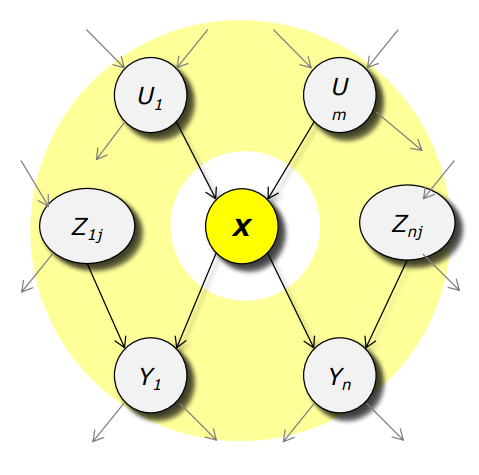
\includegraphics[width=0.5\textwidth]{./img/Reti/MarkovBlanket.png}
    \caption{I nodi $U_i, Z_{ij}, Y_j$ appartengono alla Markov Blanket di $X$}
    \label{fig:MarkovBlanket}
\end{figure}

Una possibile procedura per la costruzione incrementale della componente topologica
di una rete Bayesiane è la seguente:
\begin{itemize}
    \item Scegliere un insieme di variabili $\{x_1, \dots, x_n\}$ che rappresentano
          le variabili del dominio.
    \item Scegliere un ordinamento topologico per le variabili.
    \item Inizializzare il numero dei nodi aggiunti alla rete a $i = 1$.
    \item Selezionare la variabile $X_i$ e aggiungere il nodo corrispondente alla
          rete.
          \begin{itemize}
              \item Porre $parents(X_i)$ uguale all'insieme minimale di nodi,
                    appartenenti alla rete nel momento corrente $\{X_{(1)} \dots X_{(i-1)}\}$
                    che soddisfa la proprietà di indipendenza condizionale.
              \item Computare la CPT per la variabile $X_i$.
          \end{itemize}
    \item Incrementare il numero dei nodi aggiunti alla rete $i=i+1$. E ripetere il
          procedimento per ogni variabile.
\end{itemize}
Il metodo di costruzione delle reti è un passo fondamentale per la corretta
rappresentazione del dominio. La scelta delle relazioni di dipendenza condizionale
impatta notevolmente sulla quantità di parametri che devono essere specificati
per la rete.

Oltre a costituire una rappresentazione completa e non ridondante di un dominio
una Rete Bayesiana è spesso molto più compatta dell'intera distribuzione di
probabilità congiunta. Questo rende possibile il trattamento di domini
caratterizzati da un numero molto elevato di variabili.

La compattezza delle Reti Bayesiane è un esempio della proprietà dei sistemi
strutturati localmente o sparsi. In ogni sistema strutturato localmente ogni
sotto-componente interagisce solo con un numero limitato di altre componenti,
indipendentemente dal numero totale di componenti del sistema.

La strutturazione locale è di norma associata ad un fattore di crescita della
complessità lineare e non esponenziale. Nel caso di una Rete Bayesiana è 
ragionevole ipotizzare che ogni variabile sia direttamente influenzata da al 
massimo $k$ variabili.

Nel caso in cui si consideri una Rete Bayesiana costituita da $n$ variabili
Booleane avremo che la quantità di informazione necessaria per specificare una
qualsiasi CPT è limitata superiormente da $2^k$ numeri per cui la rete completa
richiede di specificare al più $n \cdot 2^k$ numeri. Mentre specificare l'intera
distribuzione congiunta di probabilità richiede $2^n$ numeri.
\subsection{Indipendenza condizionata}
Esiste un metodo per scoprire se in una rete Bayesiana due variabili sono
condizionalmente indipendenti. Questo metodo prende il nome di \textbf{D-separazione}.
\begin{definizione}[\textbf{D-separazione}]
    Due nodi $X$ e $Z$ sono \textbf{D-separati} da un insieme $E$ di variabili con
    evidenza se e solo se ogni cammino non orientato da $X$ a $Z$ è \textbf{bloccato}
\end{definizione}
\begin{definizione}[\textbf{cammino bloccato}]
    Un cammino è \textbf{bloccato} se e solo se vale almeno una delle seguenti
    condizioni:
    \begin{itemize}
        \item Se esiste una variabile $V$ tale che appartiene alle evidenze e
              gli archi del camino sono \textbf{tail-to-tail}.
              \begin{figure}[!ht]
                  \centering
                  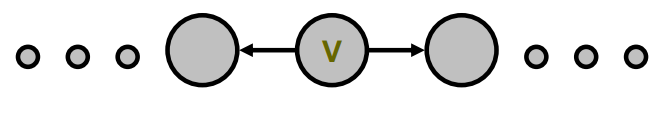
\includegraphics[width=0.5\textwidth]{./img/Reti/TailToTail.png}
                  \caption{Collegamento tail-to-tail}
                  \label{fig:tail-to-tail}
              \end{figure}
        \item Se esiste una variabile $V$ tale che appartiene alle evidenze e
              gli archi che collegano $V$ sono \textbf{tail-to-head}.
              \begin{figure}[!ht]
                  \centering
                  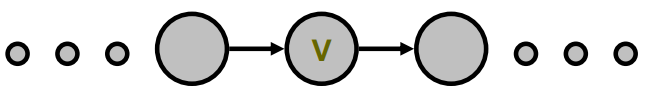
\includegraphics[width=0.5\textwidth]{./img/Reti/TailToHead.png}
                  \caption{Collegamento tail-to-head}
                  \label{fig:tail-to-head}
              \end{figure}
        \item Se esiste una variabile $V$ tale che la variabile e tutti i suoi figli
              \textbf{non} appartengono ad $E$ e gli archi che collegano $V$ al
              resto del cammino sono \textbf{head-to-head}.
              \begin{figure}[!ht]
                  \centering
                  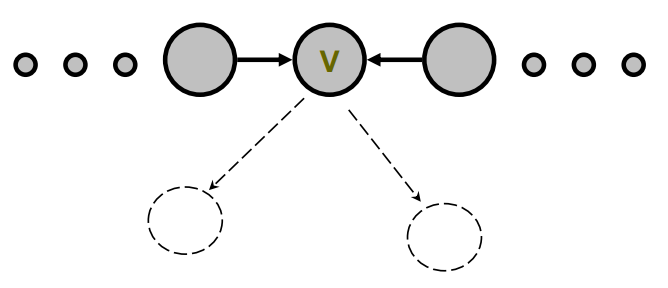
\includegraphics[width=0.5\textwidth]{./img/Reti/HeadToHead.png}
                  \caption{Collegamento head-to-head}
                  \label{fig:head-to-head}
              \end{figure}
    \end{itemize}
\end{definizione}
La d-separazione può essere calcolata in tempo lineare. Quindi abbiamo a
disposizione un algoritmo efficiente per inferire automaticamente se apprendere
il valore di una variabile può fornirci delle informazioni aggiuntive su altre
variabili, date le informazioni a disposizione.
\begin{teorema} [\textbf{Verma \& Pearl}]
    Se in una rete Bayesiana un insieme di variabili $E$ di evidenza D-separa
    $X$ e $Z$, allora $X$ e $Z$ sono indipendenti.
\end{teorema}
\begin{definizione}[\textbf{d-connessione}]
    Due variabili sono \textbf{d-connesse} se e solo se non sono d-separate
\end{definizione}
Per testare se le variabili sono condizionalmente indipendenti si può usare il
\textbf{processo di moralizzazione}:
\begin{enumerate}
    \item \textbf{Disegnare grafo ancestrale}: rete composta delle variabili
          citate e tutti i loro predecessori.
    \item \textbf{Moralizzare il grafo}: per ogni coppia di variabili che hanno
          un figlio in comune, si traccia un arco non orientato tra di loro, in
          caso di più genitori si collegano le coppie a due a due.
    \item \textbf{Disorientiamo il grafo}: sostituzione degli archi orientati
          con archi non orientati
    \item \textbf{Eliminiamo i given e gli archi incidenti}: eliminare i nodi
          facenti parte dell'evidenza e tutte le connessioni.
\end{enumerate}
Se al termine di questo processo si hanno:
\begin{itemize}
    \item \textbf{Variabili disconnesse}: è garantito che le variabili sono
          indipendenti
    \item \textbf{Variabili connesse}: non è garantito che le variabili siano
          indipendenti.
\end{itemize}
\begin{esempio}
    Vediamo ora un esempio del processo di moralizzazione. Vogliamo verificare
    se $A$ e $B$ sono condizionalmente indipendenti dati $D$ e $F$.
    \begin{figure}[!ht]
        \centering
        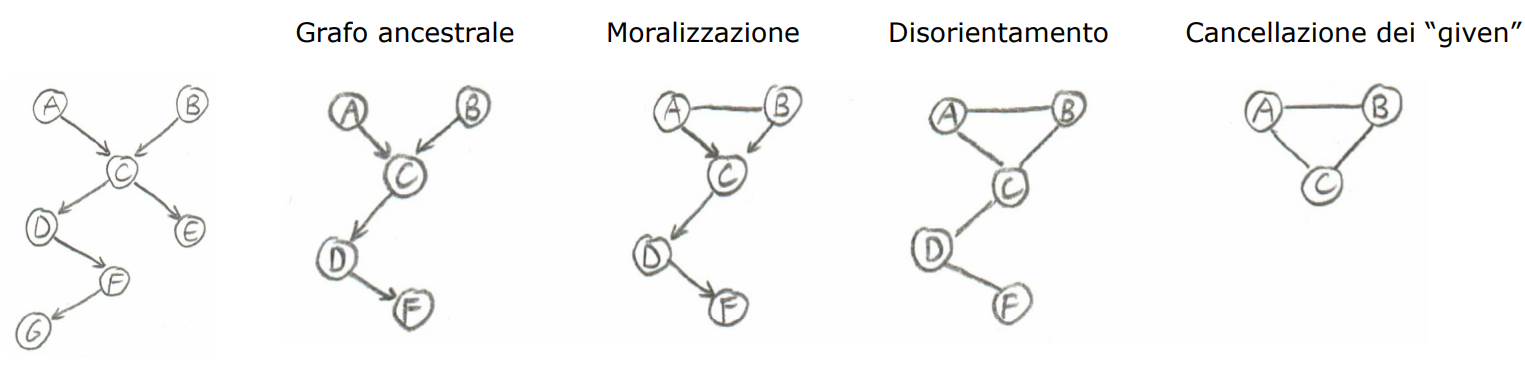
\includegraphics[width=1\textwidth]{./img/Reti/Moralizzazione.png}
        \caption{Esempio di moralizzazione}
        \label{fig:moralizzazione}
    \end{figure}
\end{esempio}
\subsection{Distribuzioni condizionali}
Per ridurre il numero di parametri nelle CPT possiamo utilizzare le \textbf{distribuzioni
    canoniche} per rappresentare dei pattern standard tra i parametri come per
i nodi deterministici. Si possono utilizzare le distribuzioni canoniche solo
quando si possono notare dei pattern particolari, ex: and tra genitori, or tra
genitori, somma dei genitori$\dots$

Una volta identificato il pattern, questo ci permette di specificare un numero 
limitato di parametri per compilare la CPT, dal momento che alcuni si derivano 
con le distribuzioni canoniche.
\begin{definizione}[\textbf{Nodo deterministico}]
    Un \textbf{nodo deterministico} è caratterizzato dal fatto che il valore che
    esso assume è completamente determinato tramite il valore assunto dai suoi
    genitori. Non c'è incertezza.
\end{definizione}
Le relazioni tra genitori e figli possono essere di diversi tipi:
\begin{itemize}
    \item \textbf{Logiche}: come ad esempio l'\texttt{OR} tra le variabili dei genitori.
    \item \textbf{numeriche}: come ad esempio il \texttt{minimo} valore delle
          variabili dei genitori.
\end{itemize}
Un importante pattern è l'\textbf{indipendenza di uno specifico contesto} ovvero
quando la probabilità condizionata di un nodo è condizionalmente indipendente
da alcuni genitori dati certi valori di altri (if-else sintax).

Le relazioni incerte, possono essere caratterizzate dalle \textbf{Noisy Logical
    Relations} che permettono di modellare l'incertezza dei genitori nel causare
il figlio. Queste relazioni sono utili per modellare situazioni in cui la presenza
di un genitore non implica necessariamente la presenza del figlio.
Andiamo per esempio ad analizzare il modello \textbf{Noisy-OR}. Questo modello 
consente di introdurre incertezza circa la capacità di ogni nodo genitore di 
causare il valore vero della variabile figlio. 

Il modello Noisy-OR effettua le seguenti ipotesi:
\begin{itemize}
    \item Tutte le possibili cause sono note
    \item L'inibizione di un genitore è indipendente dall'inibizione degli altri
          genitori per il nodo considerato.
\end{itemize}
In questo caso specifico la probabilità di un determinato evento, è data dal 
prodotto delle probabilità di inibizione per ogni nodo genitore.
\subsection{Rappresentazioni efficiente delle distribuzioni continue}
Per rappresentare efficientemente i nodi di distribuzioni continue, usando quelle
canoniche, possiamo pensare di discretizzare le variabili continue definendo un
insieme finito di intervalli. Il problema che sorge utilizzando questo approccio
è legato alla perdita di informazioni sul dato. Inoltre, le CPT spesso aumentano 
di dimensione.

Una soluzione alternativa è rappresentare le variabili con delle \textbf{funzioni
    di densità di probabilità} vengono descritte tramite un numero finito e di
norma contenuto di parametri. Un esempio è la funzione di densità di probabilità
della distribuzione normale, la quale viene completamente specificata tramite
la media e la deviazione standard.
\begin{definizione}[\textbf{Rete Bayesiana Ibrida}]
    Una rete che contiene nodi discreti e continui prende il nome di \textbf{Rete
        Bayesiane Ibrida}
\end{definizione}
Per specificare una Rete Bayesiana Ibrida dobbiamo definire due nuovi tipi di
distribuzione:
\begin{itemize}
    \item La distribuzione condizionale di una variabile continua dati i genitori
          discreti o continui.
    \item La distribuzione condizionale di una variabile discreta dati i genitori
          continui.
\end{itemize}

\section{Inferenza}
L'obiettivo fondamentale è quello di riuscire a calcolare la posterior di un insieme 
di variabili considerando una serie di variabili di evidenza.

\begin{itemize}
    \item $X$ sarà la variabile di query
    \item $E$ insieme di variabili di evidenza
    \item $e$ specifico evento, ovvero un assegnamento congiunto dei singoli valori
    delle variabili di evidenza
    \item $Y$ insieme di variabili non di evidenza
\end{itemize}

L'insieme complessivo di variabili è $V = \{X\} \cup E \cup Y$. 
Una tipica query della quale bisogna calcolare la posterior è
$$P(X | E = e)$$
Prima chiedevamo di calcolare la distribuzione di probabilità della viabile date 
tutte le altre variabili nella rete.

Nelle reti bayesiane abbiamo diverse tipologia di inferenza:
\begin{itemize}
    \item \textbf{diagnostica}: si passa dagli effetti alle cause, l'evidenza è 
    nei discendenti e l'informormazione sale dai figli ai genitori.
    \item \textbf{causale}: si passa dalle cause agli effetti, l'evidenza è 
    nei genitori e l'informormazione scende dai genitori ai figli.
    \item \textbf{intercausale}: si passa l'informazione tra cause ed effetti comuni
    \item \textbf{mista}: l'informazione è presente sia nel genitore sia nel figlioe 
    quindi abbiamo sia una una componente diagnostica sia una componente intercausale
\end{itemize}

Inserire l'evidenza nella rete allora significa che si devono aggiurnare tutte le 
CPT della rete bayesiana. Quindi implementare il meccanismo inferenza data una 
evidenza allora significa inserire l'evidenza che aggiorna le CPT e successivamente 
si possono evvettuare tutte le query che si vogliono fare. La distribuzione si 
calcola facilmente perché sono state aggiornate precedentemente le CPT in base 
all'evidenza osservata.

% TODO: inserire immagini

Per rispondere ad una query generica 
$$P(X|E=e)$$
allora sfrutto la seguente equazione (algoritmo per enumerazione) 
$$P(X|E=e) = \alpha P(X,E=e) = \alpha \sum_{y} P(X,E=e, Y=y)$$
$\alpha \sum_{y} P(X,E=e, Y=y) \equiv P(X,E=e, Y=y)$ ovvero la probabilità congiunta
tra tutte le variabili, quello che effettivamente calcolavamo precedentemente. 
Si parla di enumerazione perché calcoliamo tutte le possibili combinazioni di valori
delle variabili che non fanno parte dell'evidenza.
Nota che si aggiunge la costante di normalizzazione, ovvero $\alpha = \frac{1}{\prod_{x\in X}^{max}P(X=x)}$.

$P(X,E=e, Y=y)$ la calcoleremo con la regola di fattorizzazione, come facevamo prima.

Quindi in generale 
$$P(X|E=e) = <P(X=x'|E=e), P(X=x''|E=e),\dots>$$

Quindi 
$$P(X=x'|E=e) = \alpha \sum_{y} P(X=x',E=e, Y=y) = \alpha \sum_{y} P(X=x',E=e, Y=y)$$ 
Dove $P(X=x',E=e, Y=y)$ lo calcoliamo come facevamo sempre, ovvero sia $K \in \{X, E, Y\}$
allora 
$$P(X=x',E=e, Y=y) = \prod_{K} P(K=k | parents(K))$$
Mentre $\alpha = \frac{1}{\prod_{x\in X}^{max}P(X=x)}$.

Il processo di inferenza per $n$ variabili booleane è pari a $O(n2^n)$. Possiamo 
migliorare le tempistiche in questo modo:
\begin{itemize}
    \item migliorare il calcolo $P(K=k | parents(K))$ andando a raccogliere 
    quei fattori che non dipendo dalle sommatorie e quindi rispariamo delle moltiplicazioni.
    \item dal momento che calcoliamo tutte le combinazioni dei valori delle variabili
    significa che ricalcoliamo sempre gli stessi valori, quindi cambieremo approccio
    e useremo l'algoritmo delle elimininazioni delle variabili.
\end{itemize}

L'algoritmo si basa sul principio di risolvere il calcolo delle sommatorie in 
\textbf{bottom-up}, ovvero da dx verso sx e si salvano quei valori in modo tale 
da calcolarlo senza ripetizione.


\chapter{Processi Markoviani}
\section{Processi stocastici}
Introdurremo dei modelli probabilistici che permettono di descrivere un mondo
che cambia nel corso del tempo. Per fare ciò, avremo bisogno di una serie di
variabili casuali descritte da uno stato che varia nel tempo. Le relazioni tra i
cambiamenti di stato nel tempo descrivono l'evoluzione della variabile.

Possiamo distinguere due tipologie di modelli:
\begin{itemize}
    \item \textbf{Statici}: il valore delle variabili non cambia nel tempo.
    \item \textbf{Dinamici}: il valore delle variabili cambia nel tempo. In questa
          tipologia, lo stato corrente dipende dalla storia e il processo di
          cambiamento è descritto da una serie di fotografie, o anche dette
          \textit{time slice}, ognuna delle quali contiene un insieme di variabili
          casuali.
\end{itemize}
\begin{definizione}[\textbf{Processo stocastico}]
    Un \textbf{processo stocastico} $\{X(t), t\in T\}$ è un insieme di variabili
    aleatorie che evolve nel tempo. Nello specifico, $X(t)$ rappresenta il valore
    della variabile aleatoria $X$ al tempo $t$.
\end{definizione}
Il tempo espresso dagli indici $t$ può essere continuo o discreto. Inoltre, tali
indici possono essere finiti o infiniti.

Avremo quindi diverse tipologie di processi stocastici:
\begin{itemize}
    \item Processi stocastici a tempo continuo:
          \begin{equation*}
              \{X(t), t>0\}
          \end{equation*}
    \item Processi stocastici a tempo discreto:
          \begin{equation*}
              \{X(t), t=0,1,\dots\}
          \end{equation*}
    \item Processi stocastici a stati continui:
          \begin{equation*}
              \{X(t), t=0,1,\dots\}, X(t) \text{ distribuzione continua}
          \end{equation*}
    \item Processi stocastici a stati discreti:
          \begin{equation*}
              \{X(t), t=0,1,\dots\}, X(t) \text{ distribuzione discreta}
          \end{equation*}
\end{itemize}
La variabile $X(t)$ rappresenta il valore della variabile dato dal sistema al
tempo $t$, cioè un valore che descrive uno stato del sistema al tempo $t$. Questo
stato può essere puntuale o cumulativo.
\begin{esempio}
    $X(t)$ può rappresentare il numero di visitatori fino al tempo $t$ (cumulativo),
    oppure può rappresentare il numero di visitatori al tempo $t$ (puntuale).
\end{esempio}
Un esempio di processo stocastico naive è il \textbf{Random Walk}. Questo processo
vuole formalizzare l'idea di effettuare una camminata in cui la scelta del prossimo
passo è casuale. Può essere descritto attraverso la seguente equazione:
\begin{equation*}
    X(t) = X(t-1) + \varepsilon_t
\end{equation*}
dove $\varepsilon_t \in \{-1, 1\}$,  $P(\varepsilon_t = -1) = p$ e $P(\varepsilon_t = 1) = 1- p$.
Se $p=\frac{1}{2}$ allora il processo è bilanciato, altrimenti il modello verrebbe
chiamato random walk con \textbf{drift}, in quanto il processo tende a spostarsi
nella direzione più probabile.

Un modo per generalizzare questo processo è quello di esprimere la distribuzione
$\varepsilon_t$ come continua, ad esempio $\varepsilon_t \approx N(0, 1)$. Questo
crea una casualità maggiore.

Un'altro esempio di processo stocastico è il \textbf{processo autoregressivo del
    primo ordine} (\textit{first order autoregressive process}), il quale è descritto
dalla seguente equazione:
\begin{equation*}
    X_t = \alpha X_{t-1} + b + \varepsilon_t
\end{equation*}
con $\alpha,b$ constanti, con $-1<\alpha<1$ e $\varepsilon_t \approx N(0,1)$.

I processi stocastici sono importanti perché permettono di effettuare delle
predizioni, come ad esempio, il tracking degli oggetti in movimento nei video.
Oltre al tracking, possono essere utilizzati anche per generare dei processi come
la generazioni di comportamenti casuali per le simulazioni.
\section{Catene di Markov}
I processi stocastici possono rispettare una proprietà chiamata \textbf{proprietà
    Markoviana del primo ordine}, la proprietà assicura che la distribuzione di
probabilità per tutti i possibili valori futuri del processo dipende solo dal
valore corrente e non dai valori passati o da altre informazioni.

La generalizzazione di questa proprietà specifica il fatto che la distribuzione
di probabilità per tutti i possibili valori futuri del processo dipende da una
storia finita.

Tale proprietà può essere espressa in formule come:
\begin{equation}
    P(X_{t+1} = i_{t+1 } | X_t =i_t, \dots, X_{0} = i_{0})=P(X_{t+1} = i_{t+1 } | X_t =i_t)
\end{equation}
I processi stocastici che rispettano la \textbf{proprietà Markoviana} sono detti
\textbf{processi Markoviani} e verranno rappresentati attraverso una \textbf{catena di Markov}.

Quindi un processo stocastico a tempi discreti che rispetta la proprietà Markoviana
del primo ordine è una \textbf{catena di Markov del primo ordine} se per tutti
gli stati vale:
\begin{equation*}
    P(X_{t+1} = i_{t+1 } | X_t =i_t, \dots, X_{0} = i_{0}) = P(X_{t+1} = i_{t+1 } | X_t =i_t)
\end{equation*}
dove $P(X_0 = i_0) = q_i$, mentre $q = [q_1, \dots, q_i \dots q_n]$ rappresenta la
distribuzione di probabilità iniziale degli stati. Se non si conosce tale
distribuzione, si può assumere che sia uniforme.
\begin{nota}
    Quanto descritto fino a questo momento, può essere generalizzato a più ordini.
    Per fare ciò, si considera una storia di lunghezza pari all'ordine del processo.

    Possiamo dire che si vuole rispettare la proprietà Markoviana a più ordini.
\end{nota}
Questi processi si riferiscono a stati direttamente osservabili. Esistono anche
le catene associate a stati non osservabili direttamente, in questo caso si
parlerà di \textbf{Catena di Markov nascoste}.

Se la probabilità di un certo evento è indipendente dal tempo $t$ la catena di
Markov si definisce \textbf{stazionaria} e si ha che:
\begin{equation}
    P(X_{t+1} = i_{t+1 } | X_t =i_t) = p_{ij}
\end{equation}
dove $p_{ij}$ specifica la probabilità di passare dal valore $X_t = i$ a $X_{t + 1} = j$.

Quindi le catene di Markov possono essere rappresentate da una \textbf{Matrice di
    transizione} (ad un passo), ovvero matrici quadrate di dimensione $n \times n$
con $n$ che rappresenta il numero di stati possibili.

Ogni elemento della matrice rappresenta la probabilità di passare da uno stato
all'altro.
\begin{equation*}
    P = \begin{bmatrix}
        p_{11} & p_{12} & \dots  & p_{1n} \\
        p_{21} & p_{22} & \dots  & p_{2n} \\
        \vdots & \vdots & \ddots & \vdots \\
        p_{n1} & p_{n2} & \dots  & p_{nn} \\
    \end{bmatrix}
\end{equation*}
La matrice ha i seguenti vincoli $p_{ij} \geq 0$ e $\sum_{j=0}^{n}p_{ij}=1, \forall i$.
\begin{nota}
    Per i modelli stazionari la matrice di transizione rimane identica nel tempo.
\end{nota}

La rappresentazione grafica di una \textbf{Catena di Markov} è un grafo in cui i
nodi rappresentano gli stati che la variabile può assumere ($i,j,\dots$), mentre
gli archi rappresentano la probabilità di passare da uno stato all'altro. Quindi
la matrice di transizione diventa la matrice di adiacenza del grafo.
\begin{figure}[!ht]
    \centering
    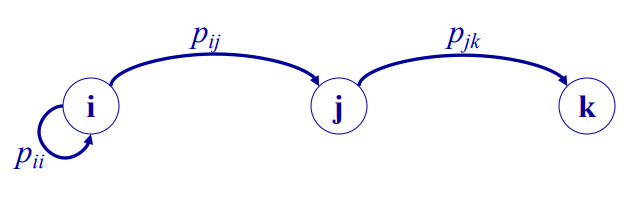
\includegraphics[width=0.5\textwidth]{img/catene/markovChain.png}
    \caption{Rappresentazione grafica di una catena di Markov}
    \label{fig:markovChain}
\end{figure}

A livello formale, per definire una \textbf{Catena di Markov} devo avere:
\begin{itemize}
    \item Un insieme di stati $S = \{S_1, S_2, \dots, S_n\}$
    \item La probabilità di transizione tra stati: $p_{ij} = P(X_{t+1} = S_i | X_t = S_j)$
    \item La distribuzione iniziale degli stati: $\pi_i = P[X_0 = S_i]$
\end{itemize}

Se non si conosce la distribuzione iniziale, allora si assume sia quella uniforme.
mentre se si conosce con certezza il valore che assume la variabile all'inizio,
allora, assumendo che $i$ sia il valore assunto da tale variabile, si avrà che
$\pi_i = 1, \forall j \neq i, \pi_j=0$.

Per calcolare la \textbf{probabilità di una serie storica} mi basta effettuare
il prodotto della probabilità di ciascuno stato dato quello precedente, sfruttando
quindi la proprietà Markoviana.
\begin{esempio}
    Se vogliamo calcolare la probabilità della serie $Sn, R,R,R,Sw,Sw$, possiamo
    usare la seguente formula:
    \begin{equation*}
        P(\langle Sn, R,R,R,Sw,Sw \rangle) = P(Sn) \cdot P(R|Sn) \cdot P(R|R)
        \cdot P(R|R)\cdot P(Sw|R) \cdot P(Sw|Sw)
    \end{equation*}
    La probabilità iniziale $P(Sn) = \pi_{Sn}$, dove $\pi$ rappresenta la
    distribuzione iniziale della variabile aleatoria.
\end{esempio}
Quando la serie storica è molto lunga il prodotto tra probabilità tende a $0$,
quindi conviene passare al logaritmo.
\subsection{Inferenza}
Possiamo effettuare inferenza di valori per istanti di tempo più lontani.

Data la matrice di transizione, possiamo calcolare la probabilità che dopo $n$
passi si trovi in uno stato specifico $j$. Per fare ciò, dovremo calcolare:
\begin{equation}
    P(X_{m + n} = j | X_{m} = i) = P(X_n = j | X_0 = i)=P_{ij}(n)
\end{equation}
dove $P_{ij}(n)$ rappresenta la probabilità di passare dallo stato $i$ allo stato
$j$ in $n$ passi. Questa probabilità può essere calcolata attraverso la seguente
formula:
\begin{equation}
    P_{ij}(n) = \prod_{i = 1}^{n} P_{ij} \equiv P^n_{ij}
\end{equation}
ovvero, si calcola il prodotto riga per colonna della matrice di transizione
per $n$ volte. In questo modo, si considerano tutti i possibili percorsi che
portano dallo stato $i$ allo stato $j$ in $n$ passi.
\begin{definizione}[\textbf{Raggiungibilità}]
    Uno stato $j$ è \textbf{raggiungibile} da uno stato $i$ se esiste un cammino
    che da $i$ arriva a $j$, in formule:
    \begin{equation*}
        P^n_{ij}>0
    \end{equation*}
    per qualche $n\geq 0$.
\end{definizione}
\begin{definizione}[\textbf{Comunicano}]
    Due stati $i$ e $j$ si dice che \textbf{comunicano} se $j$ è raggiungibile
    da $i$ e $i$ è raggiungibile da $j$. In formule:
    \begin{equation*}
        P^n_{ij}>0 \land P^n_{ji}>0
    \end{equation*}
    per qualche $n\geq 0$.
\end{definizione}
\begin{nota}
    Ogni stato comunica con se stesso per definizione e vale anche la proprietà
    transitiva.
\end{nota}
\begin{definizione}[\textbf{Irriducibilità}]
    Una catena di Markov è detta \textbf{irriducibile} se tutti i suoi stati sono
    comunicanti tra loro.
\end{definizione}
\begin{definizione}
    Un insieme di stati $S$ di una catena di Markov è un insieme \textbf{chiuso}
    se nessuno stato fuori $S$ è raggiungibile da stati in $S$.
\end{definizione}
\begin{definizione}[\textbf{Stato assorbente}]
    Uno stato $i$ si dice \textbf{assorbente} se $P_{ii} = 1$. Questo significa
    che una volta raggiunto lo stato $i$ non si può più uscire da esso.
\end{definizione}
\begin{definizione}[\textbf{Transiente}]
    Uno stato $i$ si dice \textbf{transiente} se esiste uno stato $j$ raggiungibile
    da $i$, ma $i$ non è raggiungibile da $j$. In formule:
    \begin{equation*}
        \sum_{n=1}^{\infty} P_{ii}^n < \infty
    \end{equation*}
\end{definizione}
\begin{definizione}[\textbf{Ricorrente}]
    Uno stato che non è transiente viene definito \textbf{ricorrente} se
    \begin{equation*}
        \sum_{n=1}^{\infty} P_{ii}^n = \infty
    \end{equation*}
\end{definizione}
\begin{nota}
    La ricorrenza è una proprietà di classe, se lo stato $i$ è ricorrente e
    lo stato $j$ comunica con $i$ allora $j$ è ricorrente.
\end{nota}
\begin{nota}
    Anche la transiente è una proprietà di classe.
\end{nota}
\begin{nota}
    Tutti gli stati di una catena di Markov \textbf{finita e irriducibile} sono
    anche \textbf{ricorrenti}.
\end{nota}
\begin{definizione}[\textbf{Periodicità}]
    Uno stato $i$ è \textbf{periodico} di periodo $k > 1$ se $k$ è il più piccolo
    numero tale che tutti i cammini che dallo stato $i$ ritornano ad $i$ hanno una
    lunghezza che è multiplo di $k$.
\end{definizione}
\begin{definizione}[\textbf{Aperiodico}]
    Uno stato $i$ è \textbf{aperiodico} se non è \textit{periodico}.
\end{definizione}
\begin{definizione}[\textbf{Ergodicità}]
    Se tutti gli stati della catena di Markov sono \textbf{ricorrenti}, \textbf{aperiodici}
    e \textbf{comunicano} l'un con l'altro, la catena si definisce \textbf{ergodica}.
\end{definizione}
\begin{esempio}
    Un esempio di catena \textbf{ergodica} è quella riportata in figura \ref{fig:ergodic}.
    \begin{figure}[!ht]
        \centering
        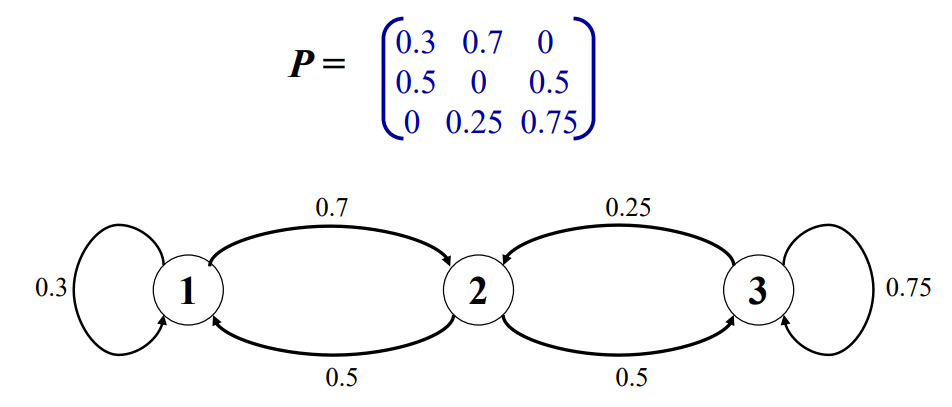
\includegraphics[width=0.5\textwidth]{img/catene/catena_ergodica.png}
        \caption{Esempio di catena ergodica}
        \label{fig:ergodic}
    \end{figure}
\end{esempio}

L'assunzione delle catene di Markov è che gli stati sono tutti direttamente osservabili,
il problema è che noi possiamo derivare la distribuzione delle variabili da delle
osservazioni su altre variabili del mondo. Significa che possiamo modificare la
distribuzione delle variabili non direttamente osservabili.
\section{Catene di Markov Nascoste}
L'evoluzione del mondo può essere modellata in modo più complesso, infatti possiamo
correggere le catene di Markov per rappresentare questa evoluzione:
\begin{itemize}
    \item $X_t$ insieme di variabili non osservabili al tempo $t$.
    \item $E_t$ insieme di variabili osservabili al tempo $t$.
    \item Dipendenze tra le variabili osservabili e non osservabili.
    \item Assunzione che i cambiamenti del mondo siano regolati da un processo
          stazionario.
    \item Assunzione di ipotesi di Markov (del primo ordine)
\end{itemize}
\begin{esempio}
    Il mio stato nascosto può essere pioggia o sole, ma non posso guardare fuori.
    Posso dedurre il tempo dalla presenza delle persone con l'ombrello bagnato o
    asciutto. Quindi osservare lo stato nascosto da altre variabili osservabili
    direttamente.
\end{esempio}
\begin{definizione}[\textbf{Catene di Markov a stati nascosti}]
    Le \textbf{catene di Markov a stati nascosti} è un processo stocastico
    continuo/discreto caratterizzato da:
    \begin{itemize}
        \item $X_t$ insieme di stati nascosti al tempo $t$
        \item $E_t$ insieme di osservazioni al tempo $t$
        \item Matrice di probabilità di transizione
              \begin{equation*}
                  P(X_t | X_{0:t-1}) = P(X_t | X_{t-1})
              \end{equation*}
        \item Matrice di probabilità di emissione delle osservazioni (sono in uno
              stato allora qual è la probabilità di osservare qualcosa)
              \begin{equation*}
                  P(E_t | X_{0:t-1}, E_{0:t-1}) = P(E_t | X_{t})
              \end{equation*}
        \item Distribuzione delle probabilità a priori a $t=0$, $P(X_0)$.
    \end{itemize}
\end{definizione}

Il modello è caratterizzato da:
\begin{itemize}
    \item \textbf{Modello di transizione}: matrice di probabilità di transizione
          di dimensione $n\times n$ ($n$ numero di stati)
          \begin{equation*}
              P(X | X_{0:t-1}) = P(X | X_{t-1})
          \end{equation*}
    \item \textbf{Modello sensoriale}: matrice di probabilità di emissione delle
          osservazioni  $n\times m$ ($n$ numero di stati, $m$ numero di osservazioni)
          \begin{equation*}
              P(E | X_{0:t-1}, E_{0:t-1}) = P(E_{t} | X_{t})
          \end{equation*}
\end{itemize}
In generale, per ogni t finito, possiamo calcolare la distribuzione congiunta:
\begin{equation}
    P(X_0, x_1,\dots,X_t, E_1,\dots, E_t) = P(X_0) \prod_{i=1}^{t}P(X_i|X_{i-1}) \cdot P(E_i|X_i)
\end{equation}
\begin{nota}
    Pensare di utilizzare questo modello per effettuare il RL per il progetto di
    sistemi complessi.

    Utilizzare lo stesso metodo per predire gli attacchi.
\end{nota}
\begin{nota}
    Per calcolare le probabilità di entrambi i modelli si effettua un conto
    numerico dal dataset.
\end{nota}

Un esempio di grafico della catena nascosta \ref{fig:HMM}.
\begin{figure}[!ht]
    \centering
    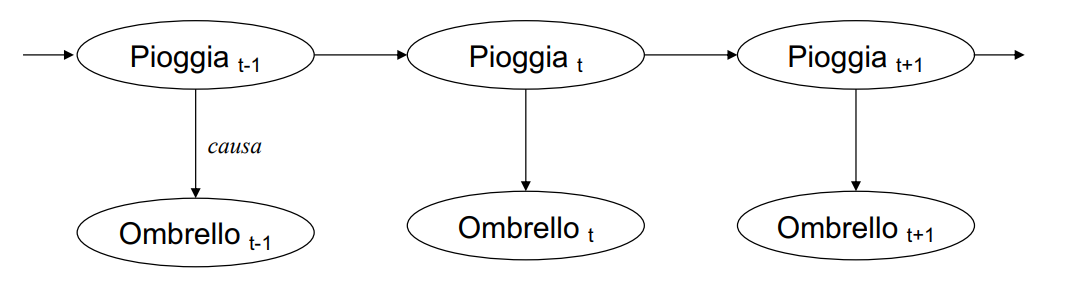
\includegraphics[width=.5\textwidth]{img/catene/hmm.png}
    \caption{Esempio di catena di Markov a stati nascosti}
    \label{fig:HMM}
\end{figure}

Secondo questo grafico potrebbero esserci problemi legati alla presenza di infinite
CPT, in realtà no perché si ha l'assunzione di \textbf{stazionarietà} (i cambiamenti
sono regolati da leggi immutabili nel tempo). In aggiunta si potrebbe pensare di
che ci siano infiniti genitori per ogni stato, in realtà no perché si ha l'assunzione
di \textbf{ipotesi di Markov} (lo stato corrente dipende solo da una storia finita
degli stati precedenti).

Si potrebbe pensare che l'\textbf{ipotesi di Markov} sia troppo stringente, per
rimediare possiamo aumentare l'ordine del modello di processo di Markov oppure di
aumentare l'insieme delle variabili di stato.
\subsection{Inferenza}
L'inferenza con questi modelli è di $4$ tipologie:
\begin{itemize}
    \item \textbf{Filtraggio}: calcolo $X_t$ dato tutte le osservazioni del
          passato $e_{1:t}$
          \begin{equation}
              P(X_t | e_{1:t})= f(e_t, P(X_{t-1}|e_{1:t-1}))
          \end{equation}
          In questo caso, le osservazioni partono da $1$, si può scegliere se
          raccoglierle da $1$ a $0$.

          Questa operazione è composta da due fasi:
          \begin{itemize}
              \item \textbf{Predizione}: calcolo della distribuzione dello stato
                    corrente al tempo $t$ dato l'osservazione fino al tempo $t-1$
                    \begin{equation}
                        P(X_t | e_{1:t-1})
                    \end{equation}
              \item \textbf{Aggiornamento}: calcolo della distribuzione dello stato
                    corrente al tempo $t$ data l'osservazione al tempo $t$:
                    \begin{equation}
                        P(e_t | X_{t})
                    \end{equation}
          \end{itemize}
          Queste due operazioni vengono unite in un unica formula:
          \begin{equation}
              P(X_{t} | e_{1:t}) = \alpha P(e_{t}|X_{t})\cdot P(X_{t}|e_{1:t-1})
          \end{equation}
          dove $\alpha$ è una costante di normalizzazione.

          La formula si ottiene prima separando l'evidenza al tempo $t$
          rispetto al tempo $t - 1$:
          \begin{equation*}
              P(X_{t} | e_{1:t}) = P(X_{t} | e_{1:t - 1}, e_{t})
          \end{equation*}
          Successivamente, utilizzando la regola di Bayes si riscrive la formula:
          \begin{equation*}
              P(X_{t} | e_{1:t - 1}, e_{t}) = \alpha P(e_{t}|X_{t}, e_{1:t-1})\cdot P(X_{t}|e_{1:t-1})
          \end{equation*}
          Infine, attraverso l'assunzione di indipendenza tra $e_{t - 1}$ e $e_{t}$
          otteniamo la formula finale.
    \item \textbf{Previsione}: coincide col filtraggio privo della fase di
          aggiornamento attraverso le osservazioni. Coincide col calcolare:
          \begin{equation}
              P(X_{t+k } | e_{1:t}) = \sum_{x_t} P(X_{t+k}|x_t) P(x_t)
          \end{equation}
          Più allunghiamo l'orizzonte di previsione, più l'incertezza aumenta,
          più breve sarà il tempo per raggiungere un punto fisso per una predizione
          (distribuzione stazionaria) e più ignoto sarà il futuro.

          Possiamo usare una ricorsione per il calcolo della verosimiglianza di
          una sequenza di osservazioni:
          \begin{equation*}
              P(e_{1:t})
          \end{equation*}
          Questa risulta utile per confrontare diversi modelli che potrebbero
          aver prodotto la stessa sequenza di osservazioni.
    \item \textbf{Smoothing}: è un processo di calcolo della distribuzione di
          stati passati, date le osservazioni fino allo stato corrente.
          \begin{equation}
              P(X_k | e_{1:t}), \forall 1 \leq k < t
          \end{equation}

          Il calcolo coincide con la seguente formula:
          \begin{equation}
              P(X_k | e_{1:t}) = P(X_k | e_{1:k}, e_{k+1:t}) = \alpha P(X_{k}|e_{1:k})
              P(e_{k+1:t}|X_k,e_{1:k}) = \alpha P(X_{k}|e_{1:k}) P (e_{k+1:t}|X_k)
          \end{equation}
          dove $\alpha$ è una costante di normalizzazione, mentre:
          \begin{itemize}
              \item $P(X_{k}|e_{1:k})$ è il filtraggio in avanti
              \item $P(e_{k+1:t}|X_k)$ è una propagazione all'indietro delle osservazioni.
          \end{itemize}
          Si sfrutta la regola di Bayes e l'indipendenza condizionata. Questa
          formula si può calcolare in modo ricorsivo.
          \begin{equation*}
              P(X_k | e_{1:t}) = \alpha P(X_{k}|e_{1:k}) P(e_{k+1:t}|X_k) = \alpha f_{1:k}b_{k+1:t}
          \end{equation*}
          dove $f_{1:k}$ consiste nel filtrare in avanti da $1$ a $k$ mentre
          $b_{k+1:t}$ viene calcolato mediante la procedura ricorsiva di backward
          che procede all'interno di $t$.
          \begin{equation}
              b_k = \alpha \cdot T \cdot E_k \cdot b_{k+1}
          \end{equation}
          dove:
          \begin{itemize}
              \item $T$ è la matrice di transizione
              \item $E_k$ è la matrice di emissione
              \item $b_{k+1}$ è il vettore di backward per il tempo $k+1$
          \end{itemize}
          Complessità spaziale molto elevata, in quanto si hanno molti stati e
          sequenze lunghe e incapacità di lavorare in ambienti online (si risolve
          con smoothing a ritardo fisso).
    \item \textbf{Spiegazione più probabile}: data una sequenza di osservazioni
          vogliamo trovare la sequenza di stati che più probabilmente ha generato
          il mio set di osservazioni.
          \begin{equation}
              \arg\max_{x_1:t} P(x_{1:t}|e_{1:t})
          \end{equation}
          Se supponiamo di avere stati binari e che la sequenza delle osservazioni
          sia lunga $n$, questo significa che abbiamo $2^n$ possibili sequenze
          di stati.

          Consideriamo ogni sequenza come un cammino lungo un grafo. La probabilità
          di ogni cammino è il prodotto delle probabilità di transizione per le
          probabilità delle osservazioni rilevate ad ogni stato.

          Infine, utilizzeremo l'algoritmo di \textbf{Viterbi}, il quale si basa
          sull'assunzione che esiste una relazione ricorsiva fra i cammini più
          probabili verso lo stato $x_{t+1}$ e i cammini più probabili verso
          ogni stato $x_t$.

          Possiamo scrivere tale relazione come:
          \begin{equation}
              \max _{x_1,\dots, x_t} P(x_1,\dots,x_t,X_{t+1}|e_{1:t+1}) = \alpha
              P(e_{t+1})\max_{x_t} \left(P(X_{t+1}|x_t)\max_{x_1,\dots,x_{t-1}}
              P(x_1,\dots,x_{t-1},x_t|e_{1:t})\right)
          \end{equation}
          dove $\alpha$ è una costante di normalizzazione.

          Riassumendo, l'algoritmo per la spiegazione più probabile è il seguente:
          \begin{itemize}
              \item Si ha una "linea" per ogni possibile stato della variabile.
              \item Per ogni stato, si calcolano tutte le probabilità con cui
                    si può raggiungere tale stato.
              \item Si calcola la probabilità di raggiungere lo stato $i$ al tempo
                    $t$ come il prodotto della probabilità di raggiungere lo stato
                    $i$ al tempo $t-1$ e la probabilità di transizione dallo
                    stato $i$ al tempo $t$.
              \item Si effettua una scelta greedy, ovvero si sceglie lo stato con
                    la probabilità maggiore e si utilizza tale probabilità per
                    effettuare i conti successivi.
              \item Per ricostruire la sequenza si parte dalla fine e si risale
                    indietro seguendo le scelte greedy effettuate.
          \end{itemize}
          % ! Metto un esempio quando torno a casa che posso disegnare sul tablet
\end{itemize}
\end{document}